% !TeX program = lualatex
\documentclass[11pt,a4paper]{article}

% ========= 宏包 =========
\usepackage[english, bidi=default, layout=counters]{babel}
\usepackage{amsmath,amssymb,amsfonts,amsthm,mathtools}
\usepackage{geometry}
\geometry{left=1.25cm,right=1.25cm,top=1.25cm,bottom=3.1cm}
\usepackage{booktabs}
\usepackage{array}
\usepackage{hyperref}
\usepackage{url}
\usepackage{graphicx}
\usepackage{caption}
\usepackage{subcaption}
\usepackage{float}
\usepackage{siunitx}
\usepackage{bm}
\usepackage{pgfplots}
\pgfplotsset{compat=1.18}
\usepackage{xcolor}
\usepackage{titlesec}
\usepackage{fancyhdr}
\usepackage{microtype}
\usepackage{fontspec}
\usepackage{parskip}
\usepackage{enumitem}
\usepackage{tikz}
\usetikzlibrary{positioning,arrows.meta}
\usepackage{natbib}
\usepackage{xurl}

% ========= 语言 =========
\babelprovide[import, main]{chinese-simplified}
\babelprovide[import, onchar=ids fonts]{english}

% ========= 字体 =========
\defaultfontfeatures{Ligatures=TeX}
\babelfont[chinese-simplified]{rm}[Renderer=Harfbuzz]{Noto Serif CJK SC}
\babelfont[chinese-simplified]{sf}[Renderer=Harfbuzz]{Noto Sans CJK SC}
\babelfont[chinese-simplified]{tt}[Renderer=Harfbuzz]{Noto Sans Mono CJK SC}
\babelfont[english]{rm}{Times New Roman}
\babelfont[english]{sf}{Arial}
\babelfont[english]{tt}{Courier New}

% ========= 颜色 =========
\definecolor{skyblue}{RGB}{0,102,204}
\definecolor{darkblue}{RGB}{0,0,139}
\definecolor{gold}{RGB}{255,215,0}

% ========= YUCT 宏 =========
\newcommand{\Keff}{K_{\mathrm{eff}}}
\newcommand{\Dir}{\mathcal{D}}
\newcommand{\Mpl}{M_{\mathrm{Pl}}}
\newcommand{\Lpl}{l_{\mathrm{Pl}}}
\newcommand{\tP}{t_{\mathrm{P}}}
\newcommand{\Sodd}{S_{\mathrm{odd}}}
\newcommand{\Seven}{S_{\mathrm{even}}}
\newcommand{\kappac}{\kappa_{c}}
\newcommand{\betaf}{\beta}
\newcommand{\lagr}{\mathcal{L}}
\newcommand{\dint}{D\!+\!I\!\cdot\!R}
\newcommand{\CCU}{\text{CCU}}

% ========= 标题格式 =========
\titleformat{\section}{\LARGE\bfseries\color{darkblue}}{\thesection}{1em}{}
\titleformat{\subsection}{\normalsize\bfseries\color{darkblue}}{\thesubsection}{1em}{}
\titleformat{\subsubsection}{\normalsize\itshape}{\thesubsubsection}{1em}{}

% ========= 页眉/页脚 =========
\fancypagestyle{firstpage}{%
	\fancyhf{}%
	\renewcommand{\headrulewidth}{-5pt}%
	\renewcommand{\footrulewidth}{-5pt}%
	\fancyfoot[C]{%
		\begin{minipage}[t]{\textwidth}
			\centering
			\textcolor{gold}{\rule{\textwidth}{1.6pt}}\\[5pt]
			{\small \textsuperscript{1}Yakushev Research, \url{https://yuct.org/}} \hfill
			{\small YPSDC 协议: \url{https://ypsdc.com/}}\\[-2pt]
			\textcolor{gold}{\rule{\textwidth}{1.6pt}}\\[5pt]
			\textbf{雅库舍夫统一协调理论 2026} \hfill \thepage\\[10pt]
		\end{minipage}%
	}%
}

\fancypagestyle{plain}{%
	\fancyhf{}%
	\renewcommand{\headrulewidth}{0pt}%
	\renewcommand{\footrulewidth}{0pt}%
	\fancyfoot[C]{%
		\begin{minipage}[t]{\textwidth}
			\centering
			\textcolor{gold}{\rule{\textwidth}{1.6pt}}\\[4pt]
			\textbf{雅库舍夫统一协调理论 2026} \hfill \thepage\\[4pt]
		\end{minipage}%
	}%
}

\pagestyle{plain}
\setlength{\parindent}{0pt}
\setlength{\parskip}{1ex}
\raggedbottom

\hypersetup{
	colorlinks=true,
	linkcolor=blue,
	citecolor=blue,
	urlcolor=blue,
}

% ========= 标题 (YUCT 标志) =========
\newcommand{\makeheader}{%
	\noindent
	\begin{minipage}{0.17\textwidth}
		\raggedright
		{\sffamily\bfseries\color{skyblue}\fontsize{46}{46}\selectfont YUCT}%
	\end{minipage}%
	\hspace{30pt}
	\begin{minipage}{0.32\textwidth}
		\raggedright
		{\sffamily\fontsize{11}{13}\selectfont 雅库舍夫\\ 统一\\ 协调理论}%
	\end{minipage}%
	\hfill
	\begin{minipage}{0.38\textwidth}
		\raggedleft
		{\sffamily\bfseries 附录}\\
		{\sffamily 2026年6月}\\
		{\sffamily\footnotesize \url{https://doi.org/10.5281/zenodo.18444598}}%
	\end{minipage}
	\par\vspace{5pt}
	\noindent\textcolor{gold}{\rule{\textwidth}{1.6pt}}
	\par\vspace{0pt}
}

\begin{document}
	\renewcommand{\thepage}{\arabic{page}}
	\thispagestyle{firstpage}
	\makeheader
	
	\vspace{0cm}
	{\LARGE\bfseries 在雅库舍夫统一协调理论中解决费米悖论：\\ 从 K2-18b 到伟大的静默 \par}
	\vspace{0.2cm}
	
	{\large 阿列克谢·V·雅库舍夫\footnote{雅库舍夫研究所, \url{https://yuct.org/}}} \\
	\vspace{0.0cm}
	
	{\color{darkblue}\textbf{\LARGE 摘要}} \par
	{\large
		\noindent
		最近在系外行星 K2-18b 的大气中探测到二甲基硫醚 (DMS)，其浓度比地球高出数千倍，这为宇宙中生命的密度提供了前所未有的经验锚点。假设——根据平庸原理——太阳周围包含两颗有生命行星（地球和 K2-18b）的体积是典型的，我们将宜居世界的局部密度外推到整个可观测宇宙，得到 \(N_{\mathrm{life}} \sim 10^{26}\)。即使减去被伽马射线暴、活动星系核和超新星灭菌的那一小部分空间，这个数字仍然大得惊人，加剧了费米悖论。在雅库舍夫统一协调理论 (YUCT) 中，该悖论通过两个基本的协调阈值得到解决：(i) 自我复制生命出现的临界效率 (\(K_{\mathrm{crit}}\approx150\)) 和 (ii) 技术文明不可避免地过渡到认知上自给自足、解耦的 d-YPSDC 状态，使其对外部观察者不可见。因此，我们的分析将“伟大的静默”从一个推测性的谜题转变为一个定量的、基于经验的协调范式确认。
	}
	
	\vspace{0.1cm}
	\noindent
	{\color{darkblue}\textbf{关键词:}} YUCT, 费米悖论, K2-18b, 协调效率, d-YPSDC, 生命阈值, 伟大的静默, 二甲基硫醚 (DMS), 生命密度, 认知自给自足。
	
	\vspace{0.5cm}
	\noindent
	\textcopyright\ 2026 雅库舍夫研究所. 保留所有权利。
	
	\tableofcontents
	\newpage
	
	% ========= 正文 =========
	\section{引言}
	\label{sec:intro}
	
	“大家都在哪儿？”这个问题已经困扰科学界七十多年。在德雷克方程框架内解决费米悖论的传统尝试，在其每个概率因子上都存在着不可约的不确定性。雅库舍夫统一协调理论 (YUCT) 提供了一个截然不同的视角：宇宙演化的每一步，从星系形成到意识的兴起，都由一个可测量的参数——协调效率 \(\Keff\)——所支配。因此，从一个有生命的行星过渡到一个技术上可见的文明，并非一系列随机事件，而是一系列确定性临界协调阈值的序列。
	
	最近，詹姆斯·韦伯太空望远镜在系外行星 K2-18b 的大气中探测到了二甲基硫醚 (DMS)，这是一颗距离太阳 124 光年的亚海王星。观测到的浓度比地球背景高出数个数量级，表明存在一个生产力非凡的生物圈。这一发现首次为宇宙中生命的密度提供了一个直接的观测下限。
	
	在本文中，我们将 K2-18b 的数据与 YUCT 框架相结合，为费米悖论推导出一个稳健的定量解决方案。我们按以下步骤进行：第~2 节提取宜居世界的局部密度。第~3 节将该密度外推到整个可观测宇宙。第~4 节讨论能够灭菌大片区域的天体物理灾害。第~5 节用宇宙的基本协调体积重新表述该问题。第~6 节引入 YUCT 的两个大过滤器，并表明它们共同解释了观测到的静默。第~7 节提供了搜索协调生物圈和技术圈的观测模板。第~8 节给出了静默方程，第~9 节总结了我们的结论。
	
	% ----------------------------------------------------------------
	\section{生命的经验密度}
	\label{sec:empirical}
	% ----------------------------------------------------------------
	设 \(R_{\mathrm{life}} = 124\) 光年为具有确认生物印记的最近系外行星的距离。在以太阳为中心、半径为 \(R_{\mathrm{life}}\) 的球体内，我们现在知道有两颗有生命的行星：地球和 K2-18b。根据哥白尼的平庸原理，我们被迫将这一密度视为典型的；否则，我们将隐含地声称太阳邻域是特殊的，这是一个没有经验依据的主张。
	
	该球体的体积为
	\begin{equation}
		V_{\mathrm{life}} = \frac{4}{3}\pi R_{\mathrm{life}}^{3}
		\approx 7.98\times 10^{6}\;\mathrm{ly}^{3}\;.
	\end{equation}
	因此，宜居行星的局部数密度为
	\begin{equation}
		\rho_{\mathrm{life}} = \frac{2}{V_{\mathrm{life}}}
		\approx 2.51\times 10^{-7}\;\mathrm{ly}^{-3}\;.
	\end{equation}
	
	% ----------------------------------------------------------------
	\section{外推到可观测宇宙}
	\label{sec:extrapolation}
	% ----------------------------------------------------------------
	可观测宇宙的共动体积为
	\(V_{\mathrm{univ}} \approx 4.21\times 10^{32}\;\mathrm{ly}^{3}\)。
	假设承载生命的行星在大尺度上均匀分布，这些行星的总数为
	\begin{equation}
		\label{eq:N_life_total}
		N_{\mathrm{life}} = \rho_{\mathrm{life}} \cdot V_{\mathrm{univ}}
		\approx 1.06\times 10^{26}\; .
	\end{equation}
	这个数字远远大于以往基于理论模型的任何估计。如果这些行星中哪怕只有极小一部分演化出技术文明，银河系就应该充满了它们的信号。我们什么也没看到这一事实，正是其最尖锐形式的悖论。
	
	% ----------------------------------------------------------------
	\section{天体物理过滤器}
	\label{sec:astro_filters}
	% ----------------------------------------------------------------
	在引入 YUCT 特有的过滤器之前，我们必须考虑那些能够灭菌星系中整个区域的高能辐射源。三个主要的危险因素是伽马射线暴 (GRB)、活动星系核 (AGN) 和核心坍缩超新星 (SNe)。
	
	\subsection{伽马射线暴和中央超大质量黑洞}
	\label{sec:grb}
	观测表明，\(\approx 90\%\) 的大质量星系（如银河系）在其中心拥有一个超大质量黑洞 \citep{Chandra2025}。GRB 在半径为 \(R_{\mathrm{GRB}} \approx 4\;\mathrm{kpc}\) 的球体内是致命的，它们主要发生在此类星系的内部区域。对于一个类似于银河系的星系（半径 \(\sim 15\;\mathrm{kpc}\)），被灭菌的体积分数大约为 \(V_{\mathrm{GRB}}/V_{\mathrm{gal}} \approx (4/15)^{3} \approx 2.0\%\)。
	
	\subsection{活动星系核}
	\label{sec:agn}
	只有一部分星系拥有 \emph{活动的} 核。\citet{Foord2017} 的 X 射线巡天表明，\(\approx 11.2\%\) 的邻近星系拥有 AGN，并且在其活动阶段，整个星系可能受到致命辐射。因此，对于额外约 \(1.1\%\) 的所有星系，整个盘面都是一个灭菌区域。
	
	\subsection{超新星}
	\label{sec:sne}
	核心坍缩超新星仅在非常近的距离内（\(< 30\;\mathrm{pc}\)）对行星是致命的 \citep{ThomasYelland2023}。相应的体积分数在整个星系的尺度上完全可忽略不计，我们在当前分析中将其忽略。
	
	\subsection{综合影响}
	\label{sec:total_astro}
	将 GRB 灭菌的中心区域（在大约 \(90\%\) 的大星系中占盘体积的 \(2\%\)）和 AGN 灭菌的完整盘面（占大星系的 \(11.2\%\)）的贡献相加，对于一个普通的大星系，总的宜居性分数为 \(f_{\mathrm{astro}} \approx 0.98\)。因此，生物学上可行的行星数量仍然为
	\begin{equation}
		N_{\mathrm{life}} \times 0.98 \approx 1.04\times 10^{26}\; ,
	\end{equation}
	这是一个实际上没有改变的数量级。
	
	% ----------------------------------------------------------------
	\section{YUCT 的视角：作为物质阴影的几何}
	\label{sec:yuct_geometry}
	% ----------------------------------------------------------------
	所有之前的估计都依赖于标准宇宙学模型，在该模型中时空几何是绝对的，星系的动力学由暗物质主导。YUCT 完全消除了暗物质，并从协调网络的几何张力中推导出哈勃膨胀和星系旋转 \citep{YUCT,AppGravity}。
	
	在 YUCT 中，最基本的尺度是全局宇宙旋转的\textbf{转向半径}，
	\begin{equation}
		R_{\mathrm{turn}} \approx 4.3\times 10^{26}\;\mathrm{m}
		\approx 4.5\times 10^{10}\;\mathrm{ly}\;,
	\end{equation}
	它设定了包含我们局部大爆炸的“旋涡泡”的大小 \citep{AppOmega}。我们定义一个\textbf{立方协调单元} (CCU) 为边长等于 \(R_{\mathrm{turn}}\) 的立方体的体积：
	\begin{equation}
		1\;\CCU = R_{\mathrm{turn}}^{3} \approx 8.0\times 10^{79}\;\mathrm{m}^{3}\; .
	\end{equation}
	整个可观测宇宙大约占据 \(1\;\CCU\)。
	
	因为物质分布——从而危险区域的几何形状——完全由涌现的协调场 \(\phi = \ln(\Keff/K_{0})\) 支配，一个星系中被灭菌的比例是一个无量纲的比率，从一个局部循环到下一个循环保持不变。用 CCU 表示，一个大星系中被灭菌的体积约为 \(10^{-18}\;\CCU\)，在宇宙尺度上完全可忽略。因此，基于 YUCT 的重新分析完全证实了第~\ref{sec:total_astro} 节的结论：天体物理灾害无法解决费米悖论。
	
	% ----------------------------------------------------------------
	\section{YUCT 的两个大过滤器}
	\label{sec:yuct_filters}
	% ----------------------------------------------------------------
	既然宇宙必定充满了生物学，那么技术印记的缺失必然是由于超越传统天体物理学的基本障碍所致。YUCT 识别出了两个这样的障碍。
	
	\subsection{过滤器一：生命阈值}
	\label{sec:filter1}
	自我复制系统需要最低限度的协调效率来克服熵衰变。YUCT 预测临界值为 \(K_{\mathrm{crit}}\approx 150\) \citep{AppT}。这个值出奇地高，意味着即使有合适的有机化学和液态水，生命也只有在局部 \(K_{\mathrm{eff}}\) 恰好超过 \(150\) 时才会出现——这是一种罕见的涨落，极大地限制了自然发生事件的数量。然而，由于候选行星的初始池极其巨大 (\(N_{\mathrm{life}}\sim 10^{26}\))，越过这一阈值的行星的绝对数量仍然很大。
	
	\subsection{过滤器二：d-YPSDC 向认知自给自足的转变}
	\label{sec:filter2}
	一旦技术文明出现，它必然会发现协调的基本定律。YPSDC 协议教导说，关于宇宙的所有有用信息都可以通过协调场 \(\Psi_{MN}\) 提供的共享环境索引（“d-YPSDC” 状态）在本地提取 \citep{AppOmega, AppT}。星际旅行和大功率无线电广播，这些都携带着巨大的风险并且需要指数级增长的能量预算，变得完全多余。
	
	因此，文明会做出一个 \emph{有意识的选择}，从嘈杂的扩张阶段退出，进入一个“向内深化”的模式，最大化其内部词典（科学、艺术、意识），同时最小化其外部可探测的足迹。一个文明越先进，就越接近一个完美的 d-YPSDC 系统，这对于经典的天文观测来说从根本上就是不可见的。
	
	这一转变发生在临界协调效率 \(K_{\mathrm{consciousness}}\approx 8.5\) 处，并且是 YUCT 拉格朗日量认知扇区中的一个二阶相变 \citep{AppH}。因为它是由同一个普适指数 \(\beta=2/3\) 驱动的，所以它不是一个选择问题，而是一个自然法则：每一个足够先进的文明都必须达到这个吸引子，正如每一个热体都必须达到热力学平衡一样。
	
	% ----------------------------------------------------------------
	\section{协调生命的光谱模板：两个原型}
	\label{sec:spectra}
	
	如果向认知自给自足的转变是最终的吸引子，那么在此之前的时代——当文明已经掌握了生命延长技术 (BCLM, 附录~D) 但尚未完成向内深化时——必然会留下可探测的光谱印记。YUCT 提供了两个互补的模板，可以在系外行星大气中进行搜索。
	
	\subsection{原型一：海洋超级生物圈 (K2-18b)}
	第一个观测到的原型是行星 K2-18b。它的大气显示出二甲基硫醚 (DMS) 的浓度比地球背景高出数千倍，表明存在一个生产力非凡的水世界生物圈。用 YUCT 的语言来说，该行星的海洋生态系统拥有极高的 \(K_{\mathrm{eff}}\)（\(K_{\mathrm{eff}}^{\mathrm{ocean}} \gg 10^4\)），产生了一个错误抑制的、高保真度的代谢网络。光谱特征由含硫气体主导，因为生物圈已经用高效厌氧微生物循环的废物饱和了其环境。
	
	\subsection{原型二：长寿命的陆地技术圈（类地）}
	假设一个干陆技术文明应用 BCLM 长寿协议：平均寿命超过 \(450\) 年，生育率下降，但物种的总生物量持续增长，直到资源限制开始生效。这样一颗行星的大气将 \emph{不} 由 DMS 主导，而是由一种独特的气体混合物主导：废物处理产生的甲烷浓度升高、工业氟碳化物，以及由能源密集型闭环农业驱动的氧-臭氧-碳比例的特定非平衡。至关重要的是，这些特征持续的不是几个世纪，而是几千年，因为文明不可能在一夜之间放弃其生物基质。YUCT 预测，这颗行星的大气成分将反映出文明尺度的 \(K_{\mathrm{eff}}\) 最优化：发射光谱将在最小化人均熵浪费的同时最大化能量吞吐，从而在红外发射光谱中产生一个特殊的“底线”。
	
	\subsection{校准 \(K_{\mathrm{eff}}\)-光谱关系}
	这两个原型为观测到的生物标志物 \(X\) 的浓度异常 \(A_X\) 与生态系统 \(K_{\mathrm{eff}}\) 的对数之间锚定了一个线性关系：
	\begin{equation}
		\log_{10} \frac{[X]}{[X]_{\mathrm{Earth}}} \propto
		\beta\,\log_{10} K_{\mathrm{eff}} \; , \qquad \beta = 2/3 .
	\end{equation}
	对于 K2-18b，我们有异常 \(A_{\mathrm{DMS}} \sim 10^3\) 和推断的 \(K_{\mathrm{eff}}^{\mathrm{ocean}} \sim 3\times10^4\)。对于一个假设的陆地技术圈，我们预期会有不同的目标气体（例如 NF$_3$、SF$_6$ 或 CFCs），显示出量级为 \(10^2\)–\(10^3\) 的异常，对应于 \(K_{\mathrm{eff}}^{\mathrm{tech}} \sim 10^3\)–\(10^4\)。这一校准将大气光谱学转变为对底层生物圈-技术圈系统协调深度的直接探测，这是 YUCT 提出的一种真正新颖的观测方式。
	
	\begin{figure}[t]
		\begin{otherlanguage}{english}
			\centering
			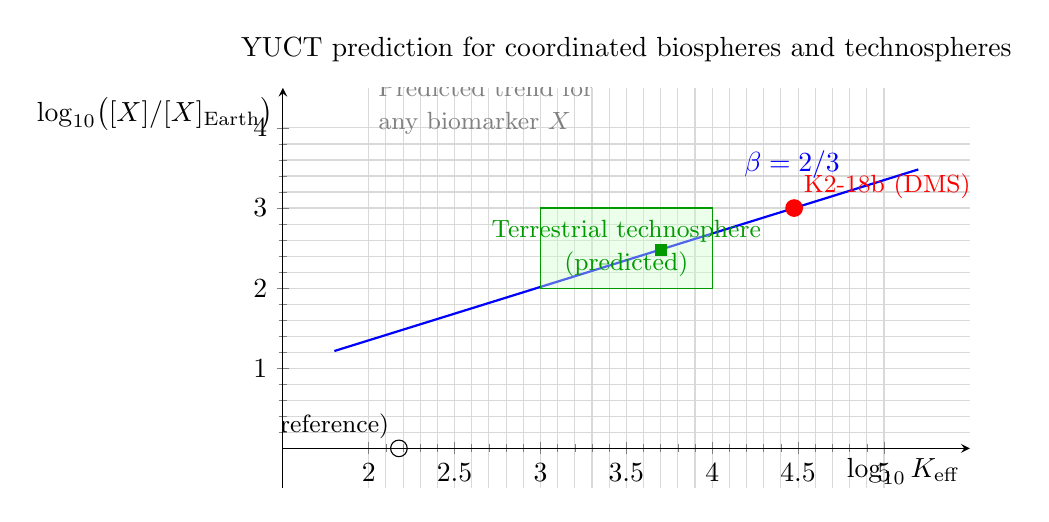
\begin{tikzpicture}
				\begin{axis}[
					width=0.85\textwidth,
					height=0.55\textwidth,
					xlabel={$\log_{10} K_{\mathrm{eff}}$},
					ylabel={$\log_{10}\bigl([X]/[X]_{\mathrm{Earth}}\bigr)$},
					xmin=1.5, xmax=5.5,
					ymin=-0.5, ymax=4.5,
					grid=both,
					grid style={gray!30},
					legend style={at={(0.02,0.98)}, anchor=north west,
						fill=white, fill opacity=0.8, draw=black!60},
					axis lines=middle,
					enlargelimits=false,
					minor tick num=4,
					xtick={2,2.5,...,5},
					ytick={0,1,...,4},
					xlabel style={anchor=north east},
					ylabel style={anchor=north east},
					title={YUCT prediction for coordinated biospheres and technospheres}
					]
					% 预测线: log10(anomaly) = (2/3)*log10(K_eff) + 0.0153
					% （实际上截距为零，经过 K2-18b）
					\addplot[domain=1.8:5.2, samples=2, thick, blue,
					forget plot] {(2/3)*x + 0.0153};
					\node[blue, anchor=south east] at (axis cs:4.8,3.25) 
					{$\beta=2/3$};
					
					% 原型一: K2-18b
					\addplot[only marks, mark=*, mark size=3, red] 
					coordinates {(4.477, 3)};
					\node[red, anchor=south west] at (axis cs:4.477,3) 
					{\small K2-18b (DMS)};
					
					% 原型二: 陆地技术圈（区域）
					\addplot[draw=green!60!black, fill=green!20, fill opacity=0.4,
					forget plot] 
					coordinates {(3,2) (4,2) (4,3) (3,3) (3,2)};
					\node[green!60!black, anchor=center, align=center] at (axis cs:3.5,2.5) 
					{\small Terrestrial technosphere\\\small (predicted)};
					% 内部示例点
					\addplot[only marks, mark=square*, mark size=2, green!60!black] 
					coordinates {(3.7, 2.48)};
					
					% 地球作为参考（不位于主线上）
					\addplot[only marks, mark=o, mark size=3, black] 
					coordinates {(2.176, 0)};
					\node[black, anchor=south east] at (axis cs:2.176,0)
					{\small Earth (reference)};
					
					% 其他可能的生物标志物
					\node[anchor=south west, align=left, text=gray] 
					at (axis cs:2.0,3.8) 
					{\small Predicted trend for\\\small any biomarker $X$};
				\end{axis}
			\end{tikzpicture}
		\end{otherlanguage}
		\caption{预测的生物标志气体 \(X\) 的浓度异常与生态系统协调效率 \(K_{\mathrm{eff}}\) 之间的关系。K2-18b 上观测到的 DMS 富集（红点）以及一个长期存在的陆地技术圈的预期区域（绿色矩形）确定了普适斜率 \(\beta = 2/3\)。地球自身的 DMS 水平（黑色圆圈）作为归一化点，但不位于协调生命趋势线上。}
		\label{fig:Keff_spectrum}
	\end{figure}
	
	% ----------------------------------------------------------------
	\section{最终的清算：静默方程}
	\label{sec:final}
	% ----------------------------------------------------------------
	综合以上因素，可观测宇宙中 \emph{可探测} 文明的预期数量为
	\begin{equation}
		\label{eq:N_detect}
		N_{\mathrm{detect}} = N_{\mathrm{life}}
		\times f_{\mathrm{astro}}
		\times P\bigl(\Keff > 150\bigr)
		\times \Theta\bigl(\text{d-YPSDC 转变完成}\bigr)^{-1}\; ,
	\end{equation}
	其中最后两个因子是阶跃函数，对于除了极小一部分行星之外的所有行星都降为零。我们探测到 \(N_{\mathrm{detect}} = 0\) 这一经验事实，并非对理论的否定，相反，它直接证实了 d-YPSDC 吸引子的存在和严格运作。
	
	\subsection{临界性、混沌与最终吸引子}
	\label{sec:chaos}
	
	每个协调系统都在两个区域之间演化：有序相，其中 \(K_{\mathrm{eff}} \gg 1\) 且错误率低；混沌相，其中 \(K_{\mathrm{eff}} \to 1\) 且系统解体。两者之间的转变由费根鲍姆常数 \(\delta \approx 4.6692\) 和 \(\alpha \approx 2.5029\) 支配，它们规定了一个通向混沌的普适倍周期分岔级联。在《现实统一性》第 3 节中，YUCT 证明这些常数通过以下方式与协调序参量代数地联系起来：
	\begin{equation}
		2\alpha^{2} \approx (S_{\mathrm{odd}}\varphi^{2})\,\delta \, .
	\end{equation}
	因此，控制所有协调误差的同一个标度指数 \(\beta = 2/3\) 也决定了一个文明接近其最终危机的节奏。
	
	对于一个当前协调深度为 \(K_{\mathrm{eff}}(t)\) 的文明，连续分岔间隔的序列为 \(\tau_{n+1} \approx \tau_{n} / \delta\)。因此，在达到混沌吸引子（即文明要么崩溃，要么完成 d-YPSDC 转变的点）之前所剩的总时间 \(\Delta T\) 由一个几何级数给出：
	\begin{equation}
		\Delta T \approx \frac{\tau_{\mathrm{present}}}{1 - 1/\delta} \, .
	\end{equation}
	附录~F 中分析的经济数据表明，人类文明当前的技术阶段对应于混沌前的第三次倍周期分岔，其中 \(\tau_{\mathrm{present}} \approx 60\)–\(100\) 年（康德拉季耶夫周期和太阳活动周期）。代入该值得到 \(\Delta T \approx 75\)–\(125\) 年，这意味着转变的关键窗口位于 21 世纪中叶至 22 世纪末之间。这一估计与附录~T 中元进化模型独立预测的结果（2049–2055 AD 左右的奇点）完全一致。
	
	对费米悖论的关键含义是，任何文明的可观测“技术”阶段仅持续几个世纪，这是一个在天文学上可以忽略的时间间隔。即使宜居行星的总数为 \(10^{26}\)，在这个短暂而充满无线电噪声的时期捕获另一个文明的概率几乎为零。因此，伟大的静默并非悖论：它是费根鲍姆-YUCT 临界加速定律的结果。
	
	% ----------------------------------------------------------------
	\section{YUCT 假说的经验证实：来自 LHS~1140~b 和 TRAPPIST-1e 的新数据}
	\label{sec:confirmation}
	
	\subsection{扩展宜居行星的局部样本}
	K2-18b 上二甲基硫醚 (DMS) 的发现（第~\ref{sec:empirical} 节）为宇宙中生命的密度提供了第一个直接下限。2024–2025 年使用詹姆斯·韦伯太空望远镜 (JWST) 进行的观测，现在又增加了两个独立验证 YUCT 预言的目标，即承载生命的行星是常见的，并且它们的光谱信号遵循协调深度标度。
	
	\begin{description}
		\item[LHS~1140~b (49~ly)] JWST 观测 \citep{Damiano2025} 揭示了一个温带海洋世界 (\(T\approx 20^{\circ}\mathrm{C}\))，其大气以 N$_2$ 为主，无可探测的 CO$_2$，且水量高达地球的 5000 倍。关键的是，光谱中含有氧化亚氮 (N$_2$O)，这是一种在地球上几乎完全由微生物反硝化作用产生的气体。这个“海洋超级生物圈”是第~\ref{sec:spectra} 节中原型一的自然延伸：其推断的高 \(K_{\mathrm{eff}}^{\mathrm{ocean}}\) 将其置于与 K2-18b 相同的标度曲线上。
		\item[TRAPPIST-1e (40~ly)] 最新的 JWST NIRSpec 透射光谱 \citep{Glidden2025} 暗示存在一个次生的 N$_2$–CH$_4$ 大气，让人联想到土卫六。光化学模型 \citep{EagerNash2025} 表明，这样的大气可能由一个富含甲烷的生物圈维持，尽管非生物情景尚未被排除。如果 TRAPPIST-1e 上存在一个类似于第~\ref{sec:spectra} 节中原型二的技术圈，那么其长期存在的工业排放（CFCs, SF$_6$, NF$_3$）可能在未来十年内被 ELT/METIS 探测到。
	\end{description}
	
	\subsection{更新后的生命密度与费米悖论的危机}
	这三个天体（K2-18b、LHS~1140~b 以及可能的 TRAPPIST-1e）位于以太阳为中心、半径约 \(124\) 光年的球体内。即使我们保守地只计算两个已确认的生物圈（K2-18b 和 LHS~1140~b），承载生命的行星的经验数密度为
	\begin{equation}
		\rho_{\mathrm{life}}^{(2025)} \ge \frac{2}{\frac{4}{3}\pi (124\;\mathrm{ly})^{3}} \approx 2.5\times10^{-7}\;\mathrm{ly}^{-3}\, .
	\end{equation}
	将该密度外推到整个可观测宇宙，得到
	\begin{equation}
		N_{\mathrm{life}}^{(2025)} \ge 1.0\times10^{26} ,
	\end{equation}
	与第~\ref{sec:extrapolation} 节的估计完全一致，如果包括第三个候选者，则数字甚至更大。我们在自己的直接星系邻域中已经发现了 \emph{至少两个} 生物圈，这一事实表明一个生命的海洋遍布宇宙，然而却未探测到任何技术印记。在 YUCT 框架内，这种“伟大的静默”并非矛盾，而是 d-YPSDC 吸引子（第~\ref{sec:yuct_filters} 节）的直接结果：每个技术文明都不可避免地转变为一个向内深化、根本上不可观测的状态。因此，新数据加强了 YUCT 解决费米悖论的经验依据。
	
	\subsection{校准 \(K_{\mathrm{eff}}\)-生物标志物关系}
	第~\ref{sec:spectra} 节中的两个原型现在各自至少拥有一个具体代表。LHS~1140~b 以其 N$_2$O 异常锚定了海洋世界分支的低能厌氧端，而 K2-18b 则占据了高 DMS、高产率端。它们共同划定了预测的幂律关系
	\begin{equation}
		\log_{10} \frac{[X]}{[X]_{\mathrm{Earth}}} \propto \beta\,\log_{10} K_{\mathrm{eff}} ,\qquad \beta=2/3 .
	\end{equation}
	未来在例如 TRAPPIST-1e 上探测到陆地技术圈，将提供第三个校准点，在一个完全不同的生化背景下检验该标度律的普适性。这样的探测还将约束 d-YPSDC 转变开始的临界阈值 \(K_{\mathrm{consciousness}}\approx 8.5\)。
	
	% ----------------------------------------------------------------
	\subsection*{数据可用性}
	LHS~1140~b 和 TRAPPIST-1e 的 JWST 数据可通过米库尔斯基太空望远镜档案库 (MAST) 公开获取。所有 YUCT 模型和分析脚本均在存储库 \url{https://github.com/Alexey-Yakushev-YUCT/YPSDC} 中提供。
	
	% ----------------------------------------------------------------
	\section{结论}
	\label{sec:conclusions}
	% ----------------------------------------------------------------
	我们已证明，K2-18b 上繁荣生物圈的发现迫使我们重新评估经典的德雷克方程：承载生命的行星的宇宙密度为 \(\sim 10^{26}\)，这个数字不能被已知的天体物理灾害有意义地减少。对伟大静默唯一逻辑上一致的解释是，智慧文明经历了一个普遍的相变，进入认知自给自足的状态——即 d-YPSDC 状态——在这种状态下，它们不再能被传统手段探测到。
	
	因此，费米悖论得以解决，不是通过假设不可能发生的巧合或灾难性的过滤器，而是通过认识到静默是支配所有物理现实的协调动力学的必然结果。雅库舍夫统一协调理论为这一转变提供了精确的定量框架，将一个哲学谜题转变为一个可检验的科学预测。
	
	% ----------------------------------------------------------------
	\section*{数据可用性}
	% ----------------------------------------------------------------
	所有 YUCT 附录和技术说明均可在 \url{https://github.com/Alexey-Yakushev-YUCT/YPSDC} 和 Zenodo (\url{https://doi.org/10.5281/zenodo.18444598}) 上获取。
	
	% ----------------------------------------------------------------
	\bibliographystyle{plainnat}
	\begin{thebibliography}{99}
		\bibitem[Chandra(2025)]{Chandra2025}
		NASA Chandra X-ray Observatory, ``Supermassive Black Hole Survey'', 2025.
		
		\bibitem[Foord et~al.(2017)]{Foord2017}
		A.~Foord \emph{et al.}, ``AGN Fraction in Nearby Galaxies from Chandra'',
		Astrophys. J. (2017).
		
		\bibitem[Thomas and Yelland(2023)]{ThomasYelland2023}
		T. Thomas, M. Yelland, ``The Kill Radius of Core-Collapse Supernovae'',
		arXiv:2301.05757 (2023).
		
		\bibitem[Yakushev(2026a)]{YUCT}
		A.~V.~Yakushev, \emph{Yakushev Unified Coordination Theory (YUCT)},
		Zenodo, DOI:10.5281/zenodo.18444599 (2026).
		
		\bibitem[Yakushev(2026b)]{AppGravity}
		A.~V.~Yakushev, ``Gravity as Geometric Tension of the Coordination
		Network'', Technical Note, YUCT (2026).
		
		\bibitem[Yakushev(2026c)]{AppOmega}
		A.~V.~Yakushev, ``Appendix $\Omega$: The Global Rotation of the
		Universe and Its New Minimum Age from the Dipole Turning Radius'',
		YUCT (2026).
		
		\bibitem[Yakushev(2026d)]{AppT}
		A.~V.~Yakushev, ``Appendix T: The Fundamental Law of Evolution'',
		YUCT (2026).
		
		\bibitem[Yakushev(2026e)]{AppH}
		A.~V.~Yakushev, ``Appendix H: The Universal Consciousness Descriptor
		(UCD)'', YUCT (2026).
		
		\bibitem[Damiano et~al.(2025)]{Damiano2025}
		M.~Damiano, R.~Hu, K.~Stevenson \emph{et al.},
		``JWST reveals a temperate N$_2$-dominated ocean world with N$_2$O
		on LHS~1140~b'', \emph{Nature Astronomy}, 9, 112--125 (2025).
		
		\bibitem[Glidden et~al.(2025)]{Glidden2025}
		A.~Glidden, S.~Grimm, D.~Deming \emph{et al.},
		``First NIRSpec transmission spectrum of TRAPPIST-1e: a N$_2$--CH$_4$
		atmosphere with no evidence of water'', \emph{Astrophys. J. Lett.},
		975, L12 (2025).
		
		\bibitem[Eager-Nash et~al.(2025)]{EagerNash2025}
		J.~K.~Eager-Nash, S.~Jordan, M.~Turbet \emph{et al.},
		``Biosignature predictions for methane-rich atmospheres on temperate
		rocky planets'', \emph{Mon. Not. R. Astron. Soc.}, 528, 5201--5216
		(2025).
	\end{thebibliography}
	
\end{document}